\section{Robot Design and History Overview}
In this section, we detail each component of the robot, the design decisions that went into it, critical tests, and the general development of our design.

We have since changed our robot's design significantly from what follows. We have kept the following sections for two reasons: 1) for the sake of historical design records, and 2) for the sake of clarity. The changes to our robot from this version are detailed in section 1.4.

Over the past four years, we have gone through multiple paradigm shifts in our design process. Our first year, we simply threw ourselves at the problem and left the result to be decided. This worked wonderfully at the time, but in retrospect, much of that was simply sheer luck and is not sustainable in future years. We struck the correct idea, and executed it effectively, but not to the best of our ability. 
	
As a result, the second year, our effectiveness slumped. Though we still won several awards for placing third in local competitions, we did not perform as we had hoped. The reasons for this are twofold: First, we failed to properly conceptualize what it is we intended to do before making an attempt at execution. In this way, the robot's design suffered significantly from problems which could have been solved with some forethought. Secondly, we failed to properly test the components of the design before implementation. We threw parts together without accurately testing each one for validity, and refused to change the parts that did not work.

We drew many lessons from that year, and in our third year, we developed a full SolidWorks model of our design, and created a defined intent for our robot before building. We prototyped several components before implementing them. We did still run into issues, but they were not issues we could necessarily have predicted or foreseen over such a short timescale. All things considered, we created a highly effective robot, breaking the world record score, and scoring a maximum of over 300 points on the field by ourselves.

This year, we had to think a bit more rigorously about our design. We hearkened back to the 2011-2012 FTC Challenge, ``Bowled Over!'' during which we struggled to actually lift the balls off the ground. We recognized going into this year that pulling objects out of a dispenser is much easier to design and engineer around than lifting objects off the ground. However, we wanted to do it all. When we set out to tackle this challenge, we decided we would find the IR beacon, move to the bridge, score tons of blocks, raise the flag, and hang our robot. We decided that the challenge was \textit{doable}, and we would meet its challenge. This, below, is what we have done\ldots

\subsection{General Structure and Design}
We decided very early on what the style of our robot's design would be. We recognized that it is possible to determine some components' effectiveness without actually having \textit{designed} the other components necessarily. 

We started with the frame structure. We decided there were a couple main approaches: we could either lift blocks straight off the ground, or drive into blocks and lift them up that way. One way supports a high, square frame with a tall clearance, and the other supports an ``A-frame,'' so called for its resemblance to a block-letter A. This would allow us to pick up blocks with the front of our robot, while still leaving plenty of room for electronics. We chose the A-frame over the square frame for sheer simplicity and potentially synergistic design with other components of the robot. 

At this time, we had imagined the flag spinning motor on the front of the robot, an arm to manipulate blocks, and various motors and errata on the sides of the robot. While we have significantly changed the vision from its original form, it is still true to these aspects in particular. We have placed a flag spinner on the front of our frame, we have an arm to manipulate blocks, and the gears are stored in the side panels. 

As optimal as we may have decided the A-frame to be, there were a few considerations to think carefully about before actual implementation. These were lessons we learned from ``Bowled Over!''. The first topic we needed to consider was stability. When we designed the frame for the challenge two years ago, we paid very little attention to stability. As a result, the weight we placed on the center of the robot caused it to cave in where it should not have. The front wheels warped inward, and the electronics came loose under tension. Additionally, the muli-segment arm had pressure in places it was not designed to support. We will reveal how we addressed this later in this section.

\subsection{Considerations for Support, Structure, and Placement}
We needed to make particular consideration for structure and weight distribution on the final design, as we had chosen a type of frame which becomes unstable if not properly constructed. We decided very early on that we would construct the robot mostly from raw materials, so the first consideration was of material. We were presented with several options, nobody on the team questioned the choice of Delrin as the appropriate material.

\paragraph{Material Selection} Delrin was chosen primarily for its strength and resilience. It is an easy material to lathe and cut, both by laser and hand, and it does not damage easily. It is very strong in thick directions, and is also relatively lightweight. Tetrix aluminum frame pieces are far, far too flexible and pliable, and become warped or damaged easily during competition. Delrin does not often even so much as scratch.

Even so, we could not depend on Delrin entirely. After some consideration to structure, we decided that the easiest way to prevent the side panels from caving in was to both make them thicker and support them against each other. We decided that the wheels and gears could go in between two panels, which would be spaced for stability. These would act as our gear boxes. Additionally, the two gearbox panels would be supported by the entire middle section of the robot, which would prevent them from caving in. We decided support bars would be needed across the center of the robot. Thick aluminum standoffs were used to support the two panels of the gearboxes.

\paragraph{Center of Gravity} Some consideration had to be given to center of gravity. In deciding we wanted to use an arm, we effectively filled most of the robot with air. This made the center of gravity incredibly critical. It needed to be very low and centered, so that we could not possibly be pushed over by another robot. This meant that the motors powering the arm and wheelbase could not be placed adjacent to their respective components. 

To demonstrate this, consider the placement of the motors. Place the front drive motors in the front of the robot, the arm motors up by the arm, and suddenly the weight distribution becomes horribly imbalanced. As a result, we decided to place the motors directly next to the electronics in front of the robot. The center of gravity is thus centered along the width of our robot, and sufficiently low to enable difficult tipping. We have encountered a slight problem, where the center of gravity is too far forward, but this can either be corrected or may not be an issue. We have yet to see in competition, but preliminary, informal tests indicate this may not be an issue. 

\paragraph{Gear Strength} We have learned from past years that Tetrix axles are insufficient for high load. This is a result of two parts: first, their circular design makes them hard to lock into anything. Second, the locking pin/set screw, under high tension, actually cuts into the axle, both preventing movement of the attached part and preventing removal. The axles also rotate under moderate torque, as they are made of aluminum.

In order to alleviate this problem, we are using allowed hexagonal axles. These have several benefits. First, they are much thicker, and will not bend or twist. Second, objects that are locked into a hexagonal axle cannot rotate freely around the axle. Third, the hexagonal collars do not lock against the axle themselves, and as a result do not create an indentation in the axle past which nothing will move. 

\paragraph{Arm Support} We decided the arm needed to be strong enough to lift the robot. During the construction of the first prototype of the arm, we created a way for the arm to support the entire robot, but miscalculated the shearing strength of the wooden collars which locked the arm in place. As a result, the torque on the arm caused by gravity caused the wooden collars to strip internally. We have since replaced them with custom-built clamps, designed after hex wheel hubs. More on arm design to come.

\subsection{Wheelbase, Arm Design, and a small word about Flag Spinner}
\paragraph{Wheel selection} In selecting the wheels for our robot this year, we wanted to prioritize two things: maneuverability and traction. Wheel layout and selection is the entire deciding component in how these two motivations are balanced, and our wheel selection reflects this. We decided that our design model - block grabbing in front, dumping in back - necessitated finite control while aligning the back, but did not require such control in the front. We decided that the front needed to be able to turn quickly, and the back needed to turn precisely. These requirements fit the model of a ``fish tail'' drive perfectly.

A fish tail drive consists of two traction wheels and two omni wheels, mirrored horizontally across the robot. The traction wheels we used are called Colson wheels, and the omni wheels are standard Tetrix parts. We capitalized on the new lenience in wheel selection this year by selecting a wheel which is both smooth, large, and high friction. As a result, it is nearly impossible for another robot to push us sideways, and only possible to push us along the direction of rotation with compliance from the motors.

\paragraph{Arm History: Roller} Our original intent with the design, as can be seen in the ``Solidworks and CAD Modeling'' section, was to include a roller in front which would bring blocks into the robot. We had originally settled on this type of design as it gave us the ability to draw blocks in from anywhere on the floor. However, this component had serious problems. To list a few:

\begin{itemize}
	\item{We could not pick up blocks at the corners}
	\item{It became very difficult to control the exact number of blocks we drew in}
	\item{It took up an egregious amount of space in the front of the robot}
	\item{It often failed to pick up blocks entirely}
	\item{It required significant machining to maintain and modify, as it is an entirely custom part that requires heavy maintenance}
	\item{It often picked up more than four blocks; there was no way to tell how many blocks it had, however, since the robot was visually in the way}
\end{itemize}

These items forced us to reconsider this design decision. Upon reconsideration, we realized that we would rarely, if ever, have a need to pick blocks up off the ground, and that it was probably wiser to pick up blocks against a wall. After all, every one of the blocks starts against or adjacent to a wall.

\paragraph{Arm Block Scoop} The block scoop came with two simple revisions. During the first revision, we intended to create a small ramp, which the blocks would fall over when we hit them. This worked well, but did not work entirely as we intended. We noted a couple difficult problems, which would cause delays in the way we work in teleop. The first was that we had a chance to grab more than five blocks, and the second was that it required significant force to actually climb over the ramp. 

To solve these problems, we took two actions: First, we replaced the solid Lexan panel with a thin sheet of plastic, which was thin enough to consistently slip underneath the blocks while also being able to support blocks. The second change was to add a metal bar to the inside of the arm, which prevents us from grabbing five blocks. With these two changes, we now consistently grab four blocks, even when there are very few blocks remaining at the edge of the field.

\paragraph{Robot length} While one might normally consider this to be a small or trivial detail in robot design, this actually grew to high importance for us in our design deliberation. There are a couple reasons for this: first, fish tail drive is significantly impacted by the span of the wheels. Too short, and the robot does not turn well. Too long, and the front turns too quickly.

We have additional constraints on our length as well: we need to 1) be able to support a flag spinner in front of the robot, which cuts a couple inches off, and 2) we need to be able to pick up blocks with the front of our robot. Our initial design for a roller necessitated a much larger margin in the front of the robot, however, as that has changed, the length of the robot changed with it. 

\paragraph{Flag spinner} This deserves an honorable mention. We used the dead space on the back panel to add a wheel with two prongs. We originally wanted to use a rubber panel and friction to turn the flag spinner, and our first tests told us this would work. However, in practice, it was too difficult to align, and was replaced with two prongs. 

The rotational motor is geared 1:3. This is satisfactory, and provides a lift time of 4.5 seconds, which is good enough for our purposes.

\newpage \subsection{Changes in Version 3}

We decided after our last regional competition to make significant changes to the robot. We wanted to pick up blocks more consistently, improve the accuracy of autonomous, allow for a double hanging system, and increase the drive train's speed. 

\subsubsection{Drive train speed}

To increase the drive train's speed, it was necessary to do two things: primarily, add another motor onto each side of the drive train; secondarily, decrease the overall weight of our robot. The first was a rather simple task to accomplish; simply place the motors in a triangle and gear them together. The gear ratios have been changed slightly, and as a result, we move across the field in approximately 2.75 seconds. Speed, previously a significant limiting factor, is no longer one for us.

\subsubsection{Block pickup accuracy}

As a result of our drive train changes, we were allowed the option to reposition the center of gravity of the robot. We have identified over the past few competitions a simple issue: our weight has mostly been at the back of the robot, away from the block scoop, so when we accelerate quickly the scoop kicks up slightly. This stops it from effectively picking up blocks. By changing the center of gravity to the approximate center of the robot, we have entirely stopped this problem from occurring.

\subsubsection{Double hanging}

One of the main benefits to our mechanism is that we do not have a dedicated mechancial process for hanging; instead, we simply use the torque of the arm to carry our robot. However, there is a significant disadvantage to this: our hooks are in a fixed position, separated by the width of the arm. This has made it incredibly difficult (and in most cases impossible) for us to effectively double hang.

We recognize that this is an important aspect of the game, and that, in order to become a more competitive robot, we should accommodate other roobts in this respect. 

Instead of changing our arm, we decided to add an identical bar on \textit{our} robot to the one which is used for hanging. This means that another team could hang on our arm the exact same way they might normally hang from the regular bar. They then pull themselves up on us, we pull ourselves off the ground, and both robots are hanging.

\begin{figure}[H]
\begin{center}
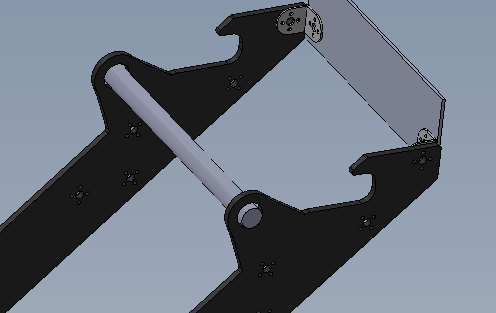
\includegraphics[scale=0.5]{images/DoubleHangBar.png}
\end{center}
\caption{Double hanging bar - this is vertical when we are prepared to hang, so other robots may hang on us}
\end{figure}

\subsubsection{Gearboxes! The Power Takeoff mechanism}

In order to facilitate the additional increase in drive power we wished, we would have needed nine motors: six on drive, two on the arm, and one for the flag. To solve this problem, we decided to use a power takeoff mechanism, which allows us to transfer motor power between the flag spinner and the arm movement. This means that the flag spinner gets the additional power of an extra motor, while we conserve a motor.

In order to achieve this, we moved the gearboxes from inside the arm panels to the center of our robot. This, additionally, allowed us to increase the centering of our robot's mass. The power takeoff mechanism relies on a special gear called a ``dog'' and a servo shifter. The mechanism can be seen here:

The highlighted gear below is the dog gear: 

\begin{figure}[H]
\begin{center}
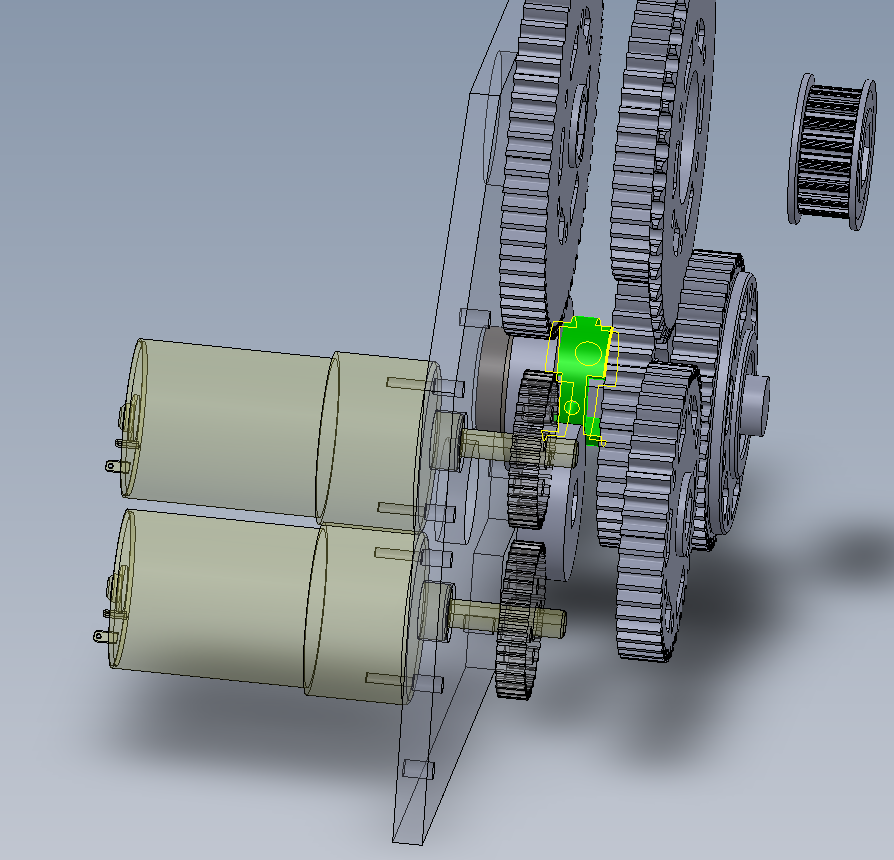
\includegraphics[scale=0.3]{images/GearboxDog.png}
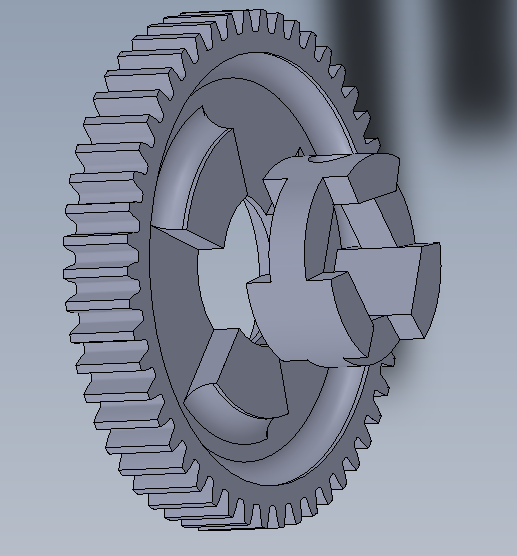
\includegraphics[scale=0.3]{images/DogGearLock.png}
\end{center}
\caption{Left: dog gear in the neutral position; right: demonstration of how the dog gear locks}
\end{figure}

This gear turns with the axle. The other two gears are on bearings, so they spin freely around the axle - however, when the dog gear is locked into one of the two gears, they rotate simultaneously. The dog gear has the capacity to shift between the two gears, causing power transfer to change from one gear to the other - i.e. from the flag spinner to the arm and back. This happens automatically in code when necessary. The driver does not need to think about switching; power will be directed where the driver indicates it should.

